\subsection{TET Features}\label{Subsec:TET_features}
% Indledning:


For each $u$ in the set of all users $U$, we build a TET $T_u$. The root of TET $T_u$ is its corresponding user $u$.
A node $n$ is a user-node in the graph $G$ if $User(n) = True$.

The feature User is in the boolean domain meaning that this feature will be either true or false (\autoref{Eq:Userdomain}).
\begin{equation}\label{Eq:Userdomain}
  User(n)\rightarrow \{True, False\}
\end{equation}


Rating is a feature which is either low, medium or high and the original rating has been split into these three categories.
The original ratings are numerical values between 0 and 5, which was then translated into the new form where $low<2.5\leq mid \leq 3.5<high$.
For each rating, we thus have that:
\begin{equation}\label{Eq:Ratingdomain}
    Rating(u, m) \rightarrow \{Low, Mid, High\}
\end{equation}
Note that \autoref{Eq:Ratingdomain} is the case for every rating in $G$.
Each genre in the dataset is a feature in the boolean domain. These features will return a value when given a movie $m$, returning true if $m$ is categorized as the genre, and false otherwise as shown in \autoref{Eq:genredomain}.
\begin{equation}\label{Eq:genredomain}
\begin{aligned}
Action(m)& \rightarrow \{True, False\} \\
Comedy(m)& \rightarrow \{True, False\} \\
&\vdots \\
Western(m)& \rightarrow \{True, False\} \\
\end{aligned}
\end{equation}

The TETs constructed from the MovieLens dataset will be represented with the structure shown in \autoref{Eq:TETstructure}.
\begin{equation}\label{Eq:TETstructure}
User(u) \stackrel{m}{\longrightarrow} Rating(u,m) \longrightarrow Genre(m)
\end{equation}

The TET will represent a neighborhood of the graph with a User as the root.

The sub-trees are themselves TETs as shown in \autoref{Eq:subtetstructure}.
\begin{equation}\label{Eq:subtetstructure}
\begin{aligned}
Rating(u,m)& \longrightarrow Action(m) \\
Rating(u,m)& \longrightarrow Comedy(m)\\
& \vdots \\
Rating(u,m)& \longrightarrow Western(m)
\end{aligned}
\end{equation}

Since the count of occurrences of \textit{False} values is often semantically not very meaningful, as stated in \cite{jaeger2019counts}, and also are of little relevance in our case, we only consider \textit{True} values. The tree will therefore end up having the form seen in \autoref{fig:Tet_example}

\begin{figure}[H]
    \centering
    \begin{adjustbox}{width=0.5\textwidth}
    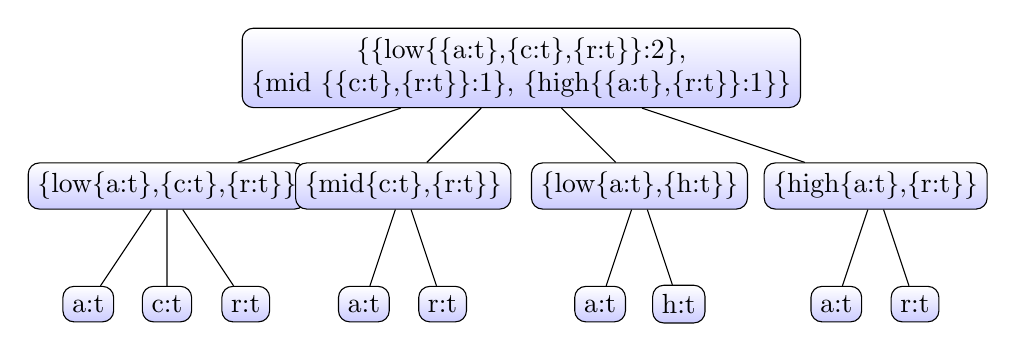
\begin{tikzpicture}[
  	every node/.style = {shape=rectangle, rounded corners,
    draw, align=center,
    top color=white, bottom color=blue!20},
    level 1/.style={sibling distance=3cm},
	level 2/.style={sibling distance=1cm}, 
    ]
  
  \node {\{\{low\{\{a:t\},\{c:t\},\{r:t\}\}:2\},\\
   \{mid \{\{c:t\},\{r:t\}\}:1\}, \{high\{\{a:t\},\{r:t\}\}:1\}\}}
	child{ node{\{low\{a:t\},\{c:t\},\{r:t\}\}} 
		child{ node{a:t}}
		child{ node{c:t}}
		child{ node{r:t}}
		}
	child{ node{\{mid\{c:t\},\{r:t\}\}} 
		child{ node{a:t}}
		child{ node{r:t}}
		}
	child{ node{\{low\{a:t\},\{h:t\}\}} 
		child{ node{a:t}}
		child{ node{h:t}}
		}
    child{ node{\{high\{a:t\},\{r:t\}\}}
	    child { node{a:t}}
      	child { node{r:t}} 
      	}
      ;
\end{tikzpicture}

%
%
%
    \end{adjustbox}
    \caption{TET Tree example}
    \label{fig:Tet_example}
\end{figure}

%The value of a TET T(X) for a user U will be denoted as V(T(U)). If the node U is not a user or is not part of domain, the value for the tree default to false.\todo{this part has to be more precise and telling look at bottom of p.39 in tet article}

The tree can also be represented as \autoref{Eq:TETvector}

\begin{equation}\label{Eq:TETvector}
    T_u=
    \begin{cases}
      (low \{(action:t),(casual:t), (romance:t)\}):2 \\
      (mid \{(comedy:t),(romance:t)\}):1 \\
      (high\{(adventure:t),(romance:t)\}):1
    \end{cases}
\end{equation}

% Where is the action and horror movie?
This tells that the tree $T_u$ has 2 movies with low rating and the genres action, casual, and romance. There is a movie rated in the mid range with genres comedy and romance, and a movie that is highly rated with genres adventure and romance.

With this structure we have a representation of user preferences.
The structures can be compared to find similarities and thereby make more trustworthy recommendations for a user.
